% !TeX encoding = UTF-8
% !TeX root = master.tex
% !TeX spellcheck = en_US

\documentclass[11pt,a4paper,twoside,openright]{report}

\usepackage[utf8]{inputenc}
\usepackage[portuguese,english]{babel}
\selectlanguage{english}

\usepackage[mieic]{styles/feupteses}
% Additional options for feupteses.sty:
% - juri: prints line numbers
% - final: final version
% - onpaper: links are not shown (for paper versions)
% - backrefs: include back references from bibliography to citation place

%\usepackage[lofdepth,lotdepth]{subfig}
\usepackage{afterpage}
\usepackage{graphicx}
\usepackage{flafter}
\usepackage{animate}
\usepackage{float}
\usepackage{grffile}

\usepackage{color}
\definecolor{cloudwhite}{cmyk}{0,0,0,0.025}

\usepackage{listings}
\lstset{ %
 language=C++,                        % choose the language of the code
 basicstyle=\footnotesize\ttfamily,
 keywordstyle=\bfseries,
 numbers=left,                      % where to put the line-numbers
 numberstyle=\scriptsize\texttt,    % the size of the fonts that are used for the line-numbers
 stepnumber=1,                      % the step between two line-numbers. If it's 1 each line will be numbered
 numbersep=8pt,                     % how far the line-numbers are from the code
 frame=tb,
 float=htb,
 aboveskip=8mm,
 belowskip=4mm,
 backgroundcolor=\color{cloudwhite},
 showspaces=false,                  % show spaces adding particular underscores
 showstringspaces=false,            % underline spaces within strings
 showtabs=false,                    % show tabs within strings adding particular underscores
 tabsize=2,	                    % sets default tabsize to 2 spaces
 captionpos=b,                      % sets the caption-position to bottom
 breaklines=true,                   % sets automatic line breaking
 breakatwhitespace=false,           % sets if automatic breaks should only happen at whitespace
 escapeinside={\%*}{*)},            % if you want to add a comment within your code
 morekeywords={*,var,template,new}  % if you want to add more keywords to the set
}

\usepackage{amsmath}
\usepackage[algochapter,linesnumberedhidden]{algorithm2e}
\usepackage{booktabs}
\usepackage{tabu}
\usepackage{rotating}
\usepackage{array}
\usepackage{multirow}
\usepackage{easylist}
\usepackage{siunitx}
\usepackage{url}
\usepackage{caption}
\usepackage{subcaption} 
\usepackage{footnote}
\usepackage{footmisc}
\usepackage{hyperref}
\usepackage[all]{hypcap}
\usepackage[noabbrev,nameinlink]{cleveref}
\usepackage{etoolbox}
\usepackage[nonumberlist,acronym,xindy]{glossaries}

\usepackage{enumitem}
\setlist{nolistsep}

\graphicspath{{figures/}}
\setcounter{tocdepth}{3}

\makeglossaries
%\usepackage[xindy]{imakeidx}
%\makeindex


\newtoggle{showcommittee}
\toggletrue{showcommittee}

%some macro definitions

% format
\newcommand{\class}[1]{{\normalfont\slshape #1\/}}

% entities
\newcommand{\Feup}{Faculdade de Engenharia da Universidade do Porto}

% abbreviations:
\newacronym{agps}{AGPS}{Assisted Global Positioning System}
\newacronym{amcl}{AMCL}{Adaptive Monte Carlo Localization}
\newacronym{api}{API}{Application Programming Interface}
\newacronym{cad}{CAD}{Computer Aided Design}
\newacronym{carlos}{CARLoS}{Cooperative Autonomous Robot for Large Open Spaces}
\newacronym{dof}{DoF}{Degrees of Freedom}
\newacronym{dgps}{DGPS}{Differential Global Positioning System}
\newacronym{ekf}{EKF}{Extended Kalman Filter}
\newacronym{esf}{ESF}{Ensemble of Shape Functions}
\newacronym{fpfh}{FPFH}{Fast Point Feature Histogram}
\newacronym{glonass}{GLONASS}{GLObalnaya NAvigatsionnaya Sputnikovaya Sistema}
\newacronym{gnss}{GNSS}{Global Navigation Satellite System}
\newacronym{gps}{GPS}{Global Positioning System}
\newacronym{gpu}{GPU}{Graphics Processing Unit}
\newacronym{icp}{ICP}{Iterative Closest Point}
\newacronym{ip}{IP}{Internet Protocol}
\newacronym{iss3d}{ISS3D}{3D Intrinsic Shape Signatures}
\newacronym{lidar}{LIDAR}{LIght Detection And Ranging}
\newacronym{mcl}{MCL}{Monte Carlo Localization}
\newacronym{ndt}{NDT}{Normal Distributions Transform}
\newacronym{opencv}{OpenCV}{Open Computer Vision library}
\newacronym{openni}{OpenNI}{Open Natural Interaction library}
\newacronym{pca}{PCA}{Principal Component Analysis}
\newacronym{pcl}{PCL}{Point Cloud Library}
\newacronym{pfh}{PFH}{Point Feature Histogram}
\newacronym{radar}{RADAR}{RAdio Detection And Ranging}
\newacronym{ransac}{RANSAC}{Random Sample Consensus}
\newacronym{ros}{ROS}{Robot Operating System}
\newacronym{rmse}{RMSE}{Root Mean Square Error}
\newacronym{sacia}{SAC-IA}{Sample Consensus Initial Alignment}
\newacronym{sc3d}{SC3D}{Shape Context 3D}
\newacronym{shot}{SHOT}{Signature of Histograms of Orientations}
\newacronym{sift}{SIFT}{Scale Invariant Feature Transform}
\newacronym{slam}{SLAM}{Simultaneous Localization And Mapping}
\newacronym{sonar}{SONAR}{SOund Navigation And Ranging}
\newacronym{tcp}{TCP}{Transmission Control Protocol}
\newacronym{toa}{ToA}{Time of Arrival}
\newacronym{tof}{ToF}{Time of Flight}
\newacronym{ttff}{TTFF}{Time To First Fix}
\newacronym{udp}{UDP}{User Datagram Protocol}
\newacronym{ukf}{UKF}{Unscented Kalman Filter}
\newacronym{usc}{USC}{Unique Shape Context}
\newacronym{xml}{XML}{Extensible Markup Language}
\newacronym{xmlrpc}{XML-RPC}{Extensible Markup Language Remote Procedure Call}

% nomenclature:
%\newglossaryentry{label}{name=$symbol$, description={multi line description}}



\begin{document}


%---------------------------------------------------------------------------------------------------
% Top matter | Information about author, supervisors and committee
%---------------------------------------------------------------------------------------------------

\title{Robot Self-Localization in Dynamic Environments}
\author{Carlos Miguel Correia da Costa}
\thesisdate{January 26, 2015}
\copyrightnotice{Carlos Miguel Correia da Costa, 2015}
\supervisor{Supervisor}{Armando Jorge Miranda de Sousa (Ph.D.)}
\supervisor{Second Supervisor}{Germano Manuel Correia dos Santos Veiga (Ph.D.)}

\iftoggle{showcommittee} {
	\committeetext{Approved in oral examination by the committee:}
	\committeemember{Chair}{Doctor Name of the President}
	\committeemember{External Examiner}{Doctor Name of the Examiner}
	\committeemember{Supervisor}{Doctor Name of the Supervisor}
	\signature
}

\logo{uporto-feup.pdf}



%---------------------------------------------------------------------------------------------------
% Prolog
%---------------------------------------------------------------------------------------------------

\begin{Prolog}
  \chapter*{Abstract}

Mobile robot platforms capable of operating safely and accurately in dynamic environments can have a multitude of applications, ranging from simple delivery tasks to advanced assembly operations. These abilities rely heavily on a robust navigation stack, which requires a stable and accurate localization system.

This dissertation describes an efficient, modular, extensible and easy to configure 3/6 DoF localization system, capable of operating on a wide range of mobile robot platforms and environments. It is able to reliably estimate the global position using feature matching and is capable of achieving high accuracy pose tracking using point cloud registration algorithms. It can use several point cloud sensing devices (such as LIDARs or RGB-D cameras) and requires no artificial landmarks. Moreover, it can update the localization map at runtime and dynamically adjust its operation rate based on the predicted robot velocity in order to use the minimum amount of hardware resources. It also offers a detailed analysis of each pose estimation, providing information about the percentage of registered inliers, the root mean square error of the inliers, the angular distribution of the inliers and outliers, the pose corrections that were performed in relation to the expected position and in case of initial pose estimation it also gives the distribution of the acceptable initial poses, which can be very valuable information for a navigation supervisor when the robot is in ambiguous areas that are very similar in different parts of the known environment.

The ROS implementation was tested in several dynamic indoor environments using two mobile robot platforms equipped with LIDARs and RGB-D cameras. Overall tests using sensor data from simulation and retrieved from the robot platforms performed in a high end laptop with an Intel Core i7 3630QM processor, 16GB DDR3 of memory and NVIDIA GTX680M graphics card, demonstrated high accuracy in complex dynamic environments, with less than 1 cm in translation error and less than 1 degree in rotation error. Execution times ranged from 5 to 30 milliseconds in a 3 DoF setup and from 50 to 150 milliseconds in a full dynamic 6 DoF configuration.

The sub centimeter accuracy achieved by the proposed localization system along with the dynamic map update capability and the need of no artificial landmarks will allow the fast deployment of mobile robot platforms capable of operating safely and accurately in cluttered environments. Moreover, the resilience to dynamic objects will grant the possibility to use robots as coworkers, helping humans perform their work more efficiently and thus reducing the overall production costs.



\chapter*{Resumo}

\begin{otherlanguage}{portuguese}

Plataformas móveis robóticas capazes de operar com precisão e de forma segura em ambientes dinâmicos têm um alargado espetro de aplicações, desde simples entregas de objetos até operações complexas de montagem. Para atingir estes requisitos de operação é necessário um sistema de navegação robusto, que por sua vez requer um módulo de localização preciso e estável.

Esta dissertação descreve um sistema de localização 3/6 DoF eficiente, modular, extensível e fácil de configurar, capaz de operar num alargado conjunto de plataformas móveis e ambientes. É capaz de estimar a posição inicial de um robô usando métodos de associação de características geométricas e consegue seguir a sua pose com alta precisão através de algoritmos de registo de nuvens de pontos. A sua implementação consegue tirar partido de vários sensores laser e câmaras RGB-D e não necessita de marcadores artificiais ou modificação do ambiente. Possui ainda a capacidade de atualizar o mapa incrementalmente e ajustar a sua frequência de funcionamento de acordo com a velocidade do robô de forma a usar o mínimo de recursos computacionais possível. Para facilitar a avaliação da qualidade da localização para operações críticas, cada estimativa da pose do robô é acompanhada com a análise do registo da nuvem de pontos, contendo informação acerca da percentagem de pontos corretamente registados, a raiz quadrada do erro quadrático médio, a distribuição angular dos pontos classificados como pertencentes e não pertencentes ao mapa de referência, as correções aplicadas à estimativa da pose e no caso de ser efetuada localização global também é disponibilizada a distribuição das poses iniciais aceitáveis, o que pode ser informação bastante útil para um supervisor de navegação quando o robô está em posições ambíguas do ambiente nas quais existe geometria semelhante em sítios diferentes do mapa.

A implementação em ROS foi testada em vários ambientes dinâmicos recorrendo a duas plataformas móveis equipadas com LIDARs e câmaras RGB-D. Os resultados obtidos usando dados de simulação e recolhidos das plataformas robóticas realizados num portátil com CPU Intel Core i7 3630QM, 16GB DDR3 de memória e placa gráfica NVIDIA GTX680M demonstraram que o sistema consegue fazer a estimativa da pose do robô com um erro de translação inferior a 1 centímetro e um erro de rotação abaixo de 1 grau. Os tempos de execução oscilaram entre 5 e 30 milissegundos para uma configuração 3 DoF e entre 50 e 150 milissegundos para 6 DoF.

A alta precisão disponibilizada pelo sistema de localização proposto em conjunto com a sua capacidade para atualizar o mapa incrementalmente e de não necessitar marcadores artificiais, irá permitir o desenvolvimento de plataformas robóticas móveis capazes de operar em ambientes não estruturados. Por outro lado, a sua robustez em relação a objetos dinâmicos abre a possibilidade dos robôs colaborarem com humanos para melhorar a produtividade global de uma dada tarefa e assim reduzir os custos de produção.

\end{otherlanguage}

  \chapter*{Acknowledgments}

I would like to express my gratitude to my supervisors and the INESC team, for their helpful contributions. Their experience and expertise significantly improved the quality of this dissertation.

I am also very grateful for the knowledge and experiences that I gather from my friends, teachers and colleagues over the years and for the brilliant work developed by the ROS and PCL community.

And of course, to my family, for their continuous support.

\vspace{10mm}
\flushleft{Carlos Miguel Correia da Costa}

  \cleardoublepage
\thispagestyle{plain}

\vspace*{8cm}

\begin{flushright}
  \textsl{``Perfection is achieved, not when there is nothing more to add, \\
           but when there is nothing left to take away.''} \\
  \vspace*{1.5cm}
           Antoine de Saint-Exupéry
\end{flushright}

  \cleardoublepage
  \pdfbookmark[0]{Table of Contents}{contents}
  \tableofcontents
  \cleardoublepage
  \pdfbookmark[0]{List of Figures}{figures}
  \listoffigures
  \cleardoublepage
  \pdfbookmark[0]{List of Tables}{tables}
  \listoftables
  \listofalgorithms
%  \glsaddall
  \printglossary[type=\acronymtype,title=Abbreviations]
  \printglossary[title=Nomenclature]
\end{Prolog}



%---------------------------------------------------------------------------------------------------
% Chapters
%---------------------------------------------------------------------------------------------------

\StartBody

\chapter{Introduction} \label{chap:introduction}



\section*{}

This chapter provides an overview about the motivations and objectives of this dissertation along with its practical applications.



\section{Context}\label{sec:introduction_context}

Humanity has sought a reliable method of navigation ever since it started to explore the world. It began with simple landmark reference points for local travels, then perfected celestial navigation for global journeys, and when it finally conquered space, it deployed a global system for high accuracy localization. Autonomous robots face the same problem, because in order to be able to navigate with precision, they first need to know their location.

Over the years, several localization methods have been proposed and refined, according to the navigation environment and the accuracy requirements. Some are meant for high precision local navigation, while others provide an approximate global position.

A robot capable of operating safely and accurately in a dynamic environment can have innumerous applications, ranging from simple delivery tasks to advanced assembly. Besides improving productivity by performing repetitive tasks with precision and speed, robots can also act as coworkers, helping humans perform their jobs more efficiently and thus, reducing the overall production costs.



\section{Project}\label{sec:introduction_project}

\gls{carlos}\footnote{\url{http://carlosproject.eu/}} is a European research project that aims to develop an autonomous robot capable of performing repetitive tasks alongside human co-workers in dynamic environments. The robot will operate in shipyards and is intended to perform fit-out operations, such as stud welding and projection mapping of \gls{cad} drawings. Stud welding is a repetitive task that provides structural support for other components, such as heat insulation layers or electrical systems. Projection mapping of \gls{cad} drawings or other important information will help human co-workers assemble components faster, because it will mark the exact position in which they must be installed.



\section{Motivation and objectives}\label{sec:introduction_goals}

With the increase of competitiveness in the current globalized trading markets, companies are trying to reduce production costs and improve the productivity of their assets. Robots can help achieve these goals by performing the simple and repetitive jobs while giving humans more free time to perform the complex and creative tasks.

Mobile platforms equipped with robotic arms provide a flexible way to automate a wide range of tasks that must be performed over large areas. However, before performing the intended operations they first need to know where they are and how they can reach the desired location. Moreover, given their limited computational resources and energy storages, they require efficient, reliable and accurate control systems capable to operate in real time.



\section{Contributions}\label{sec:introduction_contributions}

This dissertation introduces an efficient, modular and extensible 3/6 \gls{dof} localization system for mobile robot platforms capable of operating accurately and reliably in dynamic environments. It is a multi-level registration pipeline that uses geometric features to estimate the initial position of a robot platform and point cloud registration algorithms to track its pose. The tracking subsystem can have two different configurations. One tuned for maximum efficiency used for the normal operation of the mobile platform and another for unlikely situations that may require more robust registration algorithms / configurations. It also supports incremental map update and can adjust its operation rate based on the estimated robot velocity. For critical operations, it provides a detailed analysis of the tracking quality and when initial pose estimation is required it gives the distribution of the acceptable poses, which can be very valuable information if there are several areas in the known map with very similar geometry.



\section{Dissertation outline}\label{sec:introduction_structure}

The remaining of this dissertation is split over 5 chapters. \Cref{chap:localization-methods} provides an overview of the main localization methods available for mobile robot platforms. \Cref{chap:relevant-sofware-technologies} introduces the main frameworks used to implement the self-localization system. \Cref{chap:localization-system} details the architecture and \gls{ros} implementation of the proposed 3/6 \gls{dof} self-localization system. \Cref{chap:localization-system-evaluation} evaluates the results achieved with the localization system in several testing environments. Finally, \cref{chap:conclusions-and-future-work} presents the conclusions of this dissertation and suggestions for future work.

\chapter{Localization methods}\label{chap:localization-methods}



\section*{}

Self-localization is critical to any autonomous robot that must navigate the environment and requires the calculation of a 3/6 \gls{dof} pose in a given world coordinate system.

Over the years, several approaches were developed according to the precision requirements and the environment in which the robot is designed to operate. Some require support systems to calculate the position, while others are completely autonomous, allowing the robot to localize itself without any outside dependencies. Also, some systems have limited range while others can only be effective in open spaces. Moreover, several of these methods were designed to cope with errors in the localization sensors and tolerate temporary malfunctions.

The following sections will introduce some of the most used self-localization systems that can be employed in the estimation of a robot's pose.



\section{Proprioceptive methods}

Proprioceptive methods rely on internal information that the robot possesses about its own systems operation and movement in order to update the current pose estimation. As a result, they allow the robot to operate without an external support system.

Since these methods don't correct their estimations based on environment observations, they are bound to have significant cumulative errors. As such, in order to maintain an accurate estimation of a robot's pose, they are usually combined with exteroceptive systems.


\subsection{Odometry}

Odometry estimates the current pose by integrating the velocity of the robot over time. This velocity is usually calculated by measuring the number of rotations of the wheels (using optical encoders like the ones shown in \cref{fig:localization-methods_optic-encoders}). This method can provide a viable approximated location, as can be seen in \cite{Reinstein2013}.

\afterpage{
\begin{figure}[H]
	\centering
	\includegraphics*[width=0.5\textwidth]{localization_methods/optic_encoders}
	\caption[Different types of optical encoders used to measure distances]{Different types of optical encoders used to measure distances\protect\footnotemark}
	\label{fig:localization-methods_optic-encoders}
\end{figure}
\footnotetext{\url{http://www.mindspring.com/~tom2000/Delphi/Codewheel.html}}
}


\subsection{Dead reckoning}

Dead reckoning is an extension of the odometry method, in which the acceleration and angular velocity are used to improve the localization estimations.

Other sensors, such as accelerometers and gyroscopes, can also be used to improve the position estimation \cite{Ibraheem2010} and provide the robot orientation.



\section{Exteroceptive methods}

Exteroceptive methods use a range of sensors to analyze the environment and retrieve the necessary information to perform localization.


\subsection{Trilateration methods}

Trilateration is a geometric technique that can be employed in the calculation of absolute or relative positions using distances from known points.

For 3D localization, it usually involves the intersection of 4 or more spheres, in which their radius is the distance to known positions.


\subsubsection{\glsentryfirst{gnss}}

\gls{gnss} such as the \gls{gps} or \gls{glonass}, allow 3D positioning in the planet Earth  using a trilateration method \cite{Knedlik2007}.

In these systems, a constellation of satellites broadcasts a radio signal with information about its position along with the time of the message dispatch. Using this data and knowing the speed of the radio waves, the distances to the satellites can be computed.

With at least 3 satellites distances, the 3D position can be calculated, since the Earth can be used as the ${4}^{th}$ sphere (\cref{fig:localization-methods_gnss} shows a visual representation of the trilateration technique used in a global localization system).

Given that the correct measurement of the distances to the satellites relies in the accurate computation of the elapsed time between the message dispatch and its reception, it is critical that both the satellites and the receiver have synchronized clocks. This is achieved by using high precision atomic clocks in the satellites and a clock reset technique in the receiver. This reset method relies on the fact that 3 satellite distances will only have a valid location if the clock of the receiver is synchronized. With this knowledge, the receiver can compute the necessary corrections to reset its internal clock to match the satellites time.

%\afterpage{
\begin{figure}[H]
	\centering
	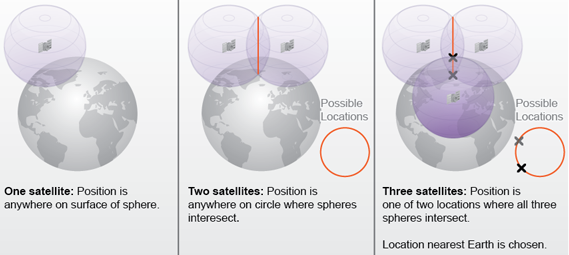
\includegraphics[width=0.8\textwidth]{localization_methods/gnss}
	\caption[Trilateration technique in a global localization system]{Trilateration technique in a global localization system\protect\footnotemark}
	\label{fig:localization-methods_gnss}
\end{figure}
\footnotetext{\url{https://www.e-education.psu.edu/geog160/node/1923}}
%}


\subsubsection{\glsentryfirst{dgps}}

The accuracy of the \gls{gps} position can be increased with the help of local broadcast stations. These stations are fixed and provide information about the corrections that can be made to the satellite signals in order to improve the localization precision.

These corrections are useful to mitigate some of the ambient interference that the satellite signals face. These interferences can range from simple signal reflection in the environment landscape to the more complex interactions with the atmosphere, which can change the speed and path of the radio signals.

The computation of the corrections \cite{Kim2007} is based on the fact that these stations are fixed, and as such, they can compare the location given by the satellite signals with their known location. With this position differential, the appropriate corrections can be calculated and broadcasted to the \gls{gps} receivers.


\subsubsection{\glsentryfirst{agps}}

\gls{agps} systems are a common method used to speed up the \gls{ttff} of a \gls{gps} receiver. They usually rely on the cellphone network to provide location estimation and signal corrections \cite{R.1948}. This information can greatly reduce the \gls{ttff} when there are few satellites visible or their signal is very weak and only temporary available.


\subsubsection{Signal strength geolocation methods}

Signal strength geolocation \cite{Kobayashi2002}, also known as fingerprinting localization \cite{Bshara2010}, is an approximate method that can be used to calculate relative positions.

It relies on the analysis of the signal attenuation from a given access point (like a Wi-Fi router or cellphone tower), to estimate distances. With enough access points (usually 4), an approximate position can be computed.

This type of distance estimation can be useful for indoor navigation, but requires a propagation model of the signal and the environment. If these models aren't accurate, then the localization precision of these methods will be very low.

Although this method is less accurate than the more recent global localization systems (such as \gls{gps}), it can be used without human made infrastructures, and as such, is a viable solution in case of temporary disruption of the \gls{gps} signal.


\subsection{Celestial navigation}

Celestial navigation \cite{Yang2011} relies on the observation of stars, planets or other reference objects, to calculate the latitude and longitude.

The calculation of the position on the surface of the Earth using celestial navigation is similar to trilateration, but in this case, angles are used instead of distances. These angles (delta), are measured between the Earth horizon and the center of the celestial object.

Having the delta, and knowing the relative position of the Earth to the reference object, along with the Greenwich hour time, it is possible to calculate a circle of position (as shown in \cref{fig:localization-methods_celestial-navigation}).

Having at least 3 circles of position, the latitude and longitude can be computed.

Although this method is less accurate than the more recent global localization systems (such as \gls{gps}), it can be used without human made infrastructures, and as such, is a viable solution in case of temporary disruption of the \gls{gps} signal.

%\afterpage{
\begin{figure}[H]
	\centering
	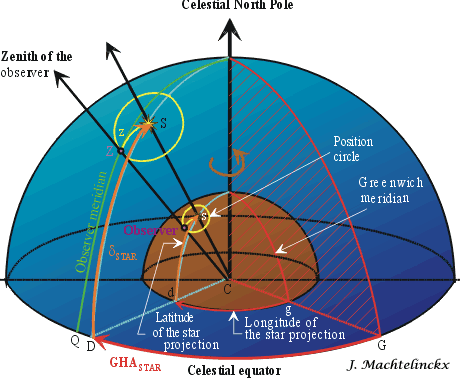
\includegraphics[width=0.45\textwidth]{localization_methods/celestial_navigation}
	\caption[Circle of position in celestial navigation]{Circle of position in celestial navigation\protect\footnotemark}
	\label{fig:localization-methods_celestial-navigation}
\end{figure}
\footnotetext{\url{http://onboardintelligence.com/CelestialNav/Celnav2.aspx}}
%}


\subsection{Landmark methods}

Landmark methods \cite{Lee2006} can be used to perform relative localization, and are very useful to reduce the required information for navigation.

In these methods a database of markers / environment geometry is stored along with its location, and when the robot recognizes one of these markers, it corrects its proprioceptive methods measures.

It is a simplification of the method that will be presented in the next section, and it is useful for environments that have unique geometry in key positions of the navigation map.


\subsection{Point cloud methods}

Point cloud localization methods can be used to perform relative localization by finding the best point cloud match between the environment and the know map (\cref{fig:localization-methods_icp} shows its application to small objects). These methods require a 2D or 3D representation of the environment and tend to be used in conjunction with proprioceptive methods (to have an estimation of movement), and also with probabilistic methods (when the point cloud acquisition location is not known).

One of the most used algorithms for 3D point cloud matching is the \gls{icp} \cite{Besl1992,Jez2008,Zhang1992,Bouaziz2013,Chetverikov2002,Djehaich2013,Zhou2011}. It is an iterative algorithm that finds the translation and rotation transformations that minimizes the distances of the corresponding points on both clouds.

There are several variants that optimize different parts of the algorithm \cite{Rusinkiewicz2001}.

The main steps for each iteration of \gls{icp} algorithm are presented below.

\begin{enumerate}
	\item  Selection of points in one or both point clouds (source and reference clouds)
	\item  Matching / pairing source points to reference points
	\item  Weighting the corresponding pairs
	\item  Rejecting low quality matches (outliers)
	\item  Assigning an error metric based on the point pairs
	\begin{enumerate}
		\item  Usually mean square error based on points distance
	\end{enumerate}
\end{enumerate}


%\afterpage{
\begin{figure}[H]
	\centering
	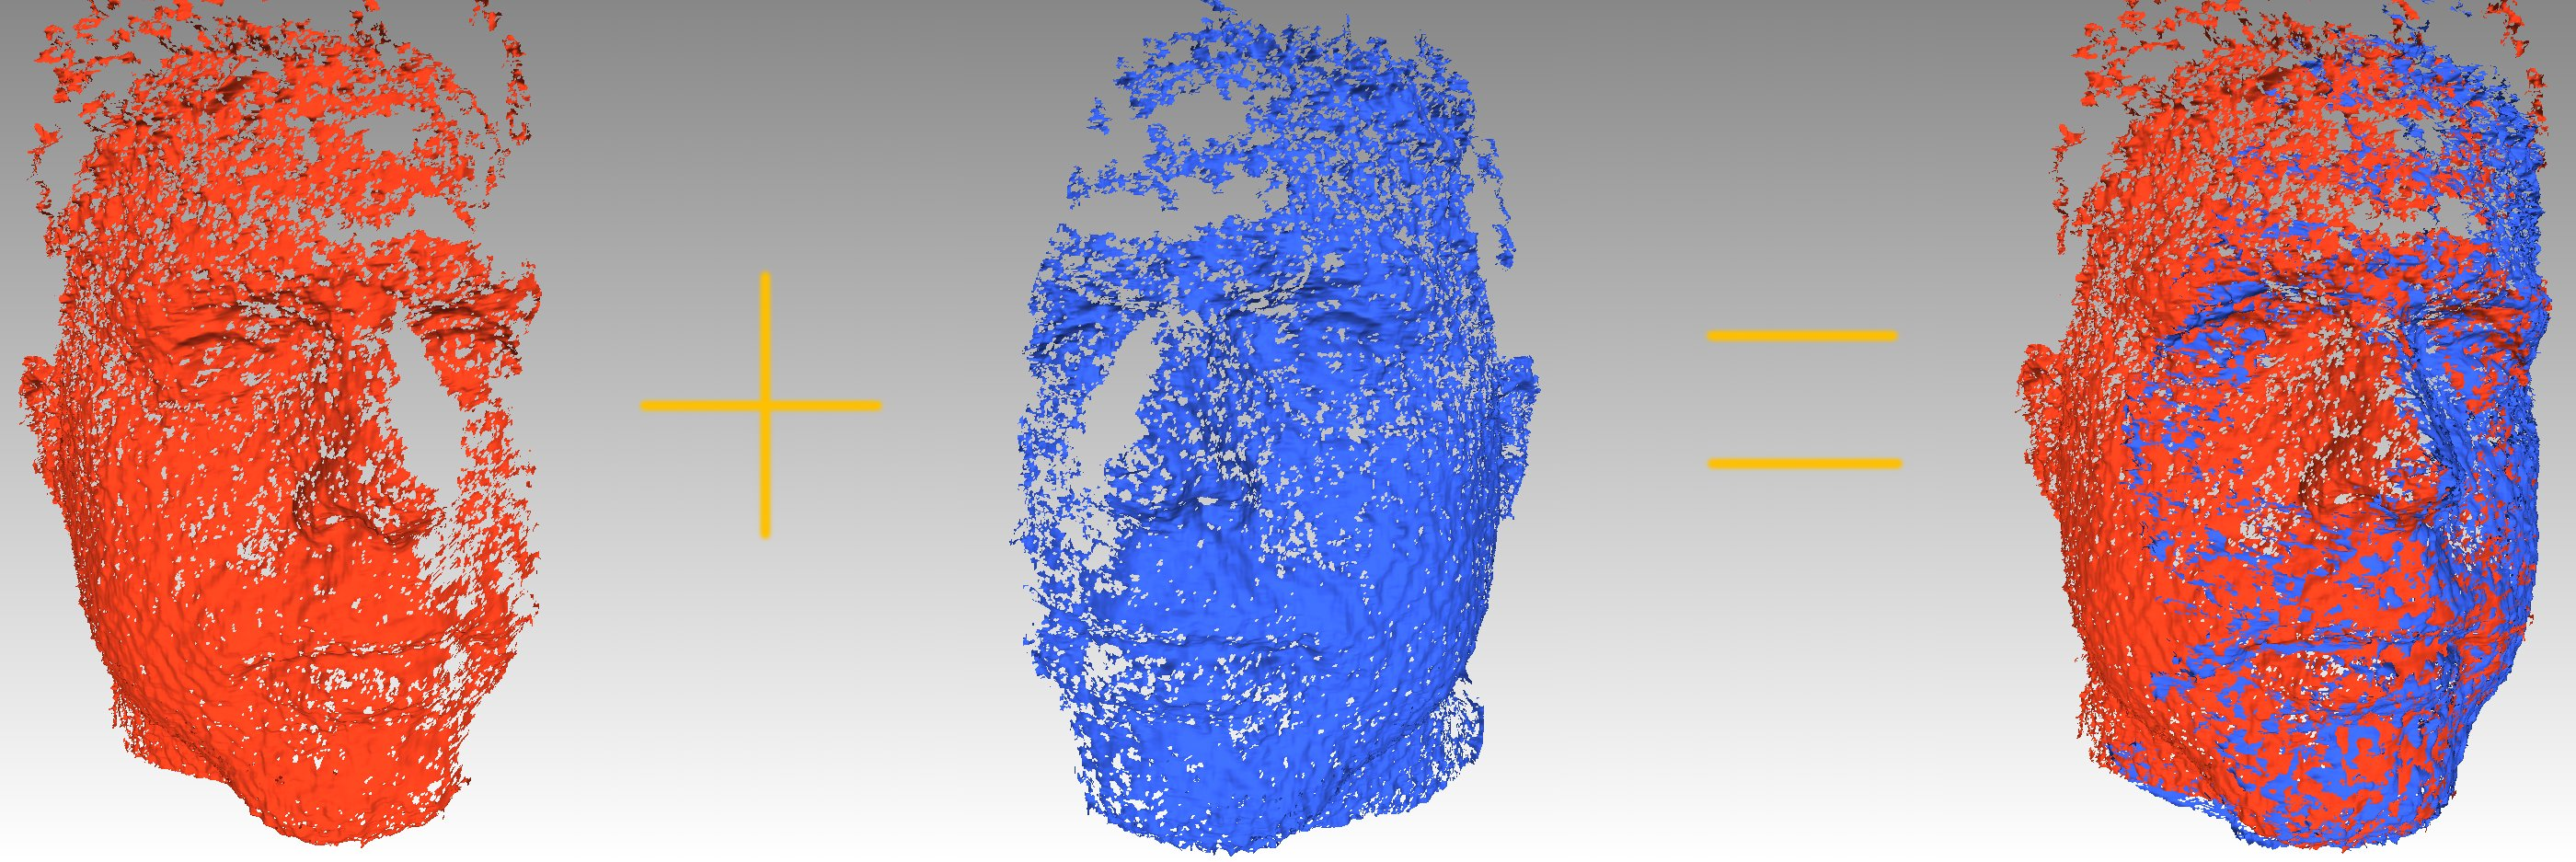
\includegraphics[width=0.75\textwidth]{localization_methods/icp}
	\caption[\glsentrytext{icp} point cloud matching]{\glsentrytext{icp} point cloud matching\protect\footnotemark}
	\label{fig:localization-methods_icp}
\end{figure}
\footnotetext{\url{http://dynface4d.isr.uc.pt/database.php}}
%}


\subsection{Probabilistic methods}

Probabilistic methods aim to reduce the impact of sensor accumulated errors or even temporary malfunctions by using Bayesian estimations and Markov processes.


\subsubsection{\glsentryfirst{mcl}}

\gls{mcl} (also known as particle filter), is a global localization algorithm that estimates the position and orientation of a robot by analyzing and adjusting the distribution and weights of state particles on a given environment \cite{Bshara2010,Arulampalam2002,Blanco2010,Chen2003b,Fox1999,Saito2009}.

It starts by randomly distributing the state particles on the map, and over time it changes their position and weight according to new sensor readings. The probable location of the robot will be in the area of the map that has the largest cluster of state particles. The figures below show the evolution of the state particles distribution during the robot movement in the environment, and illustrates how the new sensor readings changed the particles clusters\footnote{\url{http://www.cs.washington.edu/robotics/mcl/}}.

\begin{figure}[H]
	\centering
	\begin{minipage}[h]{.49\textwidth}
		\centering
		\animategraphics[width=\textwidth,loop,autoplay]{4}{localization_methods/mcl/frame-}{0}{39}
		\caption{\glsentrytext{mcl} particle distribution animation}
		\label{fig:localization-methods_mcl1}
	\end{minipage}\hfill
	\begin{minipage}[h]{.49\textwidth}
		\centering
		\includegraphics*[width=\textwidth]{localization_methods/mcl_2}
		\caption{\glsentrytext{mcl} redistribution of particles}
		\label{fig:localization-methods_mcl2}
	\end{minipage}
\end{figure}

\begin{figure}[H]
	\centering
	\begin{minipage}[h]{.49\textwidth}
		\centering
		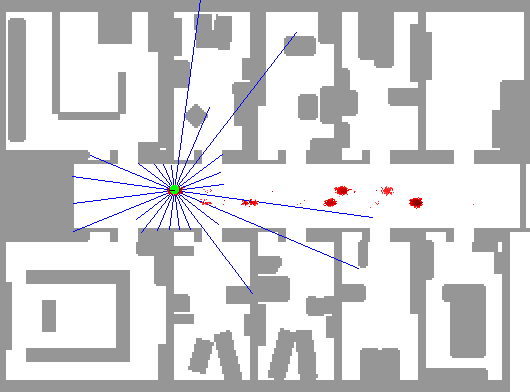
\includegraphics[width=\textwidth]{localization_methods/mcl_3}
		\caption{\glsentrytext{mcl} position refinement}
		\label{fig:localization-methods_mcl3}
	\end{minipage}\hfill
	\begin{minipage}[h]{.49\textwidth}
		\centering
		\includegraphics*[width=\textwidth]{localization_methods/mcl_4}
		\caption{\glsentrytext{mcl} position estimation}
		\label{fig:localization-methods_mcl4}
	\end{minipage}
\end{figure}


\subsubsection{Kalman filters}

Kalman filters \cite{Kalman1960} are probabilistic algorithms that estimate a given system state even when it is affected by noise or other errors. They perform linear quadratic estimations to achieve optimal results and can be efficiently implemented to be used in real time systems. They are recursive algorithms based on Marcov processes, and as a result, they only need to know the current system state in order to perform measurement corrections.

The \gls{ekf} \cite{Einicke1999,Ribeiro2004,Ivanjko2010,Liu2011} is a variant of the Kalman filter, designed to handle non-linear systems by performing linear approximations to the state variables. These approximations may lead to divergence in the estimations, and as such, the \gls{ekf} can't guarantee optimal results.

The \gls{ukf} \cite{Julier1997,Wan2002} is another variant of the Kalman filter that was designed for highly non-linear systems. It usually achieves better results than \gls{ekf} due to its unscented transform.

For the particular case of localization, these algorithms start with an initial estimation of the system state, and for each new position (computed from the sensors data), they predict the estimated robot location (according to the Bayes estimation model and the Gaussian distribution of errors), and then update their internal model of the system (mean and covariance) to incorporate the system evolution.

In \cref{fig:localization-methods_ukf} can be seen that the \gls{ukf} estimated position (red) is closer to the real position (blue) than the raw sensor measurements (green).

%\afterpage{
\begin{figure}[H]
	\centering
	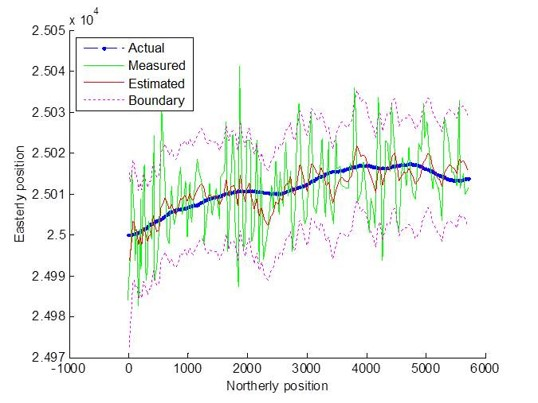
\includegraphics[width=0.9\textwidth]{localization_methods/ukf}
	\caption[Unscented Kalman Filter]{Unscented Kalman Filter\protect\footnotemark}
	\label{fig:localization-methods_ukf}
\end{figure}
\footnotetext{\url{http://www.lzcheng.com/courseworks/kalmanfilter}}
%}


\subsubsection{Perfect Match}

The Perfect Match \cite{Lauer2006a,Pinto1963} is an efficient self-localization algorithm that is largely used in the Robocup Robotic Soccer Mid Size League. Its main goal is to minimize the localization error by carefully analyzing the know map and selecting the most probable current position using a gradient descent approach. To improve tracking accuracy, the algorithm also uses a stochastic weighted approach.

With the proper configuration, it can achieve a localization accuracy similar to the particle filter, while using about ten times less computations.

An example of the position estimation can be seen in the figures below. \Cref{fig:localization-methods_pm-1} shows the probable locations when the robot detects a line on the floor, and \cref{fig:localization-methods_pm-2} illustrates their associated errors (brighter areas indicate smaller error). By using a gradient descent, the most probable location was selected (black circle).

\begin{figure}[H]
	\centering
	\begin{minipage}[h]{.495\textwidth}
		\centering
		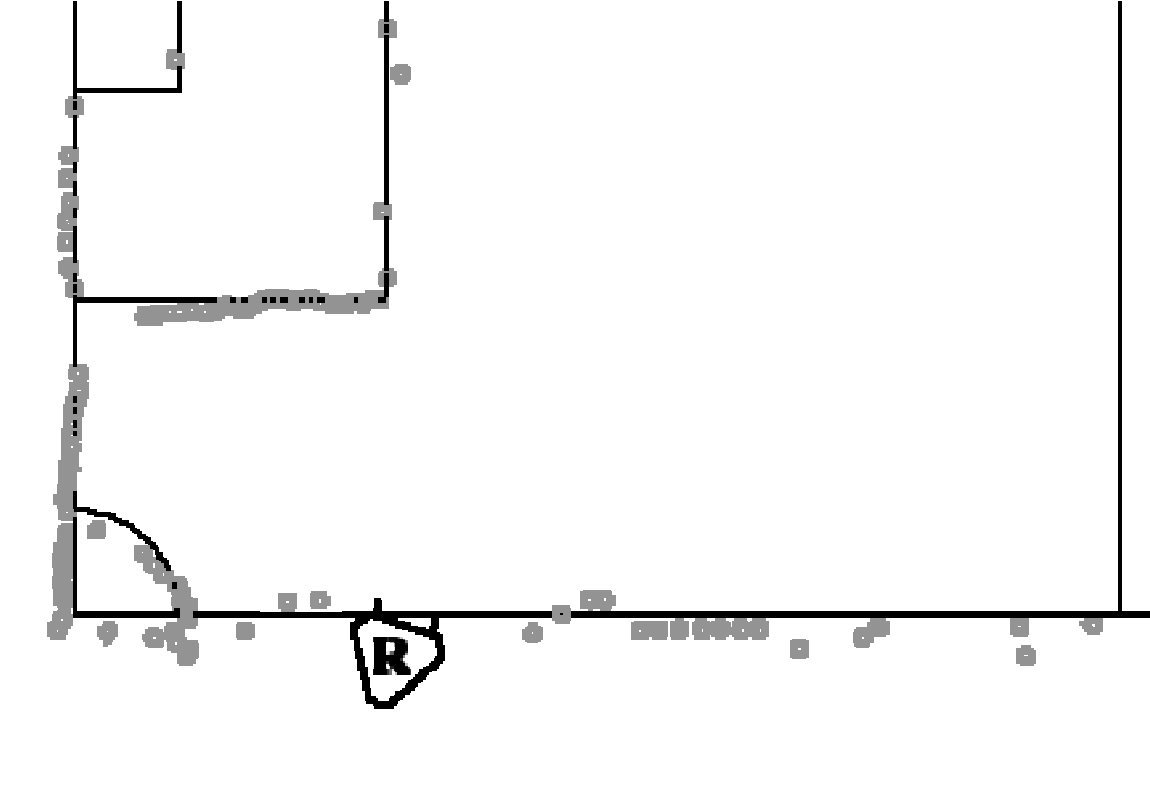
\includegraphics[width=\textwidth]{localization_methods/pm_1}
		\caption{Position estimates}
		\label{fig:localization-methods_pm-1}
	\end{minipage}\hfill
	\begin{minipage}[h]{.495\textwidth}
		\centering
		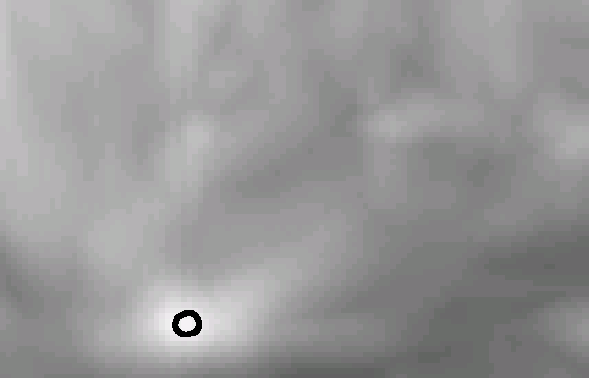
\includegraphics[width=\textwidth]{localization_methods/pm_2}
		\caption{Positions associated error}
		\label{fig:localization-methods_pm-2}
	\end{minipage}
\end{figure}


\subsection{\glsentryfirst{slam}}

\gls{slam} \cite{Thrun2002} is a very effective approach to either explore unknown environments or update a known map. It relies on both proprioceptive and exteroceptive methods to perform localization and mapping. It is also very useful to make the robot navigation more robust in dynamic environments, in which the topology of the world may change considerably over time.

There are numerous approaches to perform  \gls{slam} \cite{Tuna2012}. Some optimized for exploration and others for map improvement. For the exploration tasks, proprioceptive methods play a critical role, and are usually paired with probabilistic methods, such as Kalman filters, in order to reliably map the environment. For map correction and improvement, several probabilistic methods can be employed according to the precision required. For high accuracy 3D mapping, the \gls{icp} algorithm can be used to build accurate point clouds of the environment.



\section{Summary}

This chapter introduced several localization systems that can be used in different types of environments and with different degrees of accuracy. It started with the simple proprioceptive methods and then moved on to the more robust exteroceptive approaches.

Some techniques can be combined to improve the pose estimate or to make the localization more efficient to a particular type of environment.

For outside tasks, a \gls{gnss} approach can give accurate localization estimations with very little computation cost. On the other hand, indoor localization requires more advanced techniques in order to infer the current position based on the analysis of the robot surroundings. These techniques usually start with an estimation of the robot movement and then refine it with probabilistic or geometric methods.

\Cref{tab:localization-methods_overview-self-localization-approaches} presents an overview of the mentioned localization techniques.


\begin{sidewaystable}
	\caption{Overview of self-localization approaches}
	\tabulinesep = 0.9ex
	\centering
	\begin{tabu} { X[1.4,m,c] | X[m,c] X[m,c] X[m,c] X[m,c] X[6,m,c] }
		\rowfont{\bfseries\itshape} Method & Ideal environment & Accuracy & Operational cost & Computational cost & Notes \\
		\hline
		Odometry			& Any		& Low		& Low		& Low		& Position estimation is affected by cumulative errors \\
		Dead reckoning		& Any		& Low		& Low		& Low		& Pose estimation is affected by cumulative errors \\
		\gls{lidar}			& Any		& High		& Medium	& High		& Needs an auxiliary method to perform global localization \\
		\gls{radar}			& Any		& Medium	& High		& High		& Needs an auxiliary method to perform global localization \\
		\gls{sonar}			& Any		& Medium	& Medium	& High		& Needs an auxiliary method to perform global localization \\
		\gls{gnss}			& Outside	& Medium	& Low		& Low		& Requires a clear line of sight to at least 3 satellites \\
		Signal strength		& Any		& Low		& Low		& Low		& Requires an accurate model for the signal attenuation \\
		Celestial			& Outside	& Low		& Low		& Low		& Requires a clear view of the celestial objects and a nautical almanac \\
		Landmark			& Any		& Medium	& Low		& Medium	& Requires a database of landmarks \\
		\gls{icp}			& Indoors	& High		& Medium	& High		& Requires a detailed 3D representation of the environment \\
		\gls{mcl}			& Indoors	& Medium	& Medium	& Medium	& Inefficient for large areas \\
		Kalman filters		& Any		& Medium	& Low		& Low		& Useful to improve estimations of other methods \\
		Perfect Match		& Any		& Medium	& Low		& Low		& Not ideal for large or dynamic environments \\
		\gls{slam}			& Indoors	& Medium	& Medium	& High		& Adapts well to dynamic environments \\
	\end{tabu}
	\label{tab:localization-methods_overview-self-localization-approaches}
\end{sidewaystable}

\chapter{Relevant software technologies} \label{chap:relevant-sofware-technologies}



\section*{}

FF



\section{FF}

FF

\chapter{Point cloud algorithms}\label{chap:point-cloud-algorithms}



\section*{}

This chapter presents the main algorithms that can be used to retrieve and analyze point clouds in the context of a robot localization system.

It starts by giving an overview of how point clouds can be acquired and efficiently searched. Then moves on to the preprocessing methods that can be applied to improve the quality of the sensor data. Later on, two approaches capable of performing point cloud registration are presented. The first uses geometric features to compute the initial point cloud alignment, and the second employs error minimization techniques to calculate the final registration. Lastly it is discussed how to segment outliers and how to dynamically updated the reference point cloud using new sensor data.



\section{Point cloud acquisition}

Point clouds can be retrieved with a wide range of sensors with varying levels of precision and assembly time. They usually rely on time of flight or trilateration / triangulation techniques to compute distances to environment objects, which in combination with the sensor position and orientation allows to retrieve the Euclidean coordinates of the scene points. Some sensors can also capture the point's reflectance or color, which can be very useful in segmentation techniques and point cloud feature algorithms.


\subsection{\glsentrydesc{tof} systems}

Time of flight systems measure the time that a wave takes to leave the sensor, hit the environment and return to the sensor. Knowing the speed at which the wave travels, the distance between the two can be easily computed.

Several time of flight systems were developed over the years that use different types of waves according to the environment in which they were designed to operate. Some use high precision light waves (\gls{lidar}) while others employ less accurate radio / sound waves (\gls{radar} / \gls{sonar}). \cref{sec:localization-methods_tof-methods} gives a more detailed description of these systems.


\subsection{Triangulation and trilateration systems}

Triangulation systems measure angles to a given point from several origins in order to compute the Euclidean coordinates of an environment object. Trilateration is similar but uses distances instead of angles. These methods are useful when the sensor orientation is not known or when there are two different views of the environment (stereo cameras and structured light scanners). \Cref{sec:localization-methods_trilateration-methods} introduces some of these systems.



\section{Point cloud search data structures}

Most of the point cloud algorithms use neighbor searches to analyze the surroundings of a given point. As such, efficient data structures are needed to speedup these operations, in order to execute the algorithms efficiently.


\subsection{Voxel grids}

A voxel grid is a three dimensional space partition data structure that splits the Euclidean space into regular voxels (volume pixel). It can be built very fast but is not very efficient for sparse point clouds. \Cref{fig:point-cloud-algorithms_voxel-grid} shows how the voxel size affects the level of detail of point clouds.

\begin{figure}[H]
	\centering
	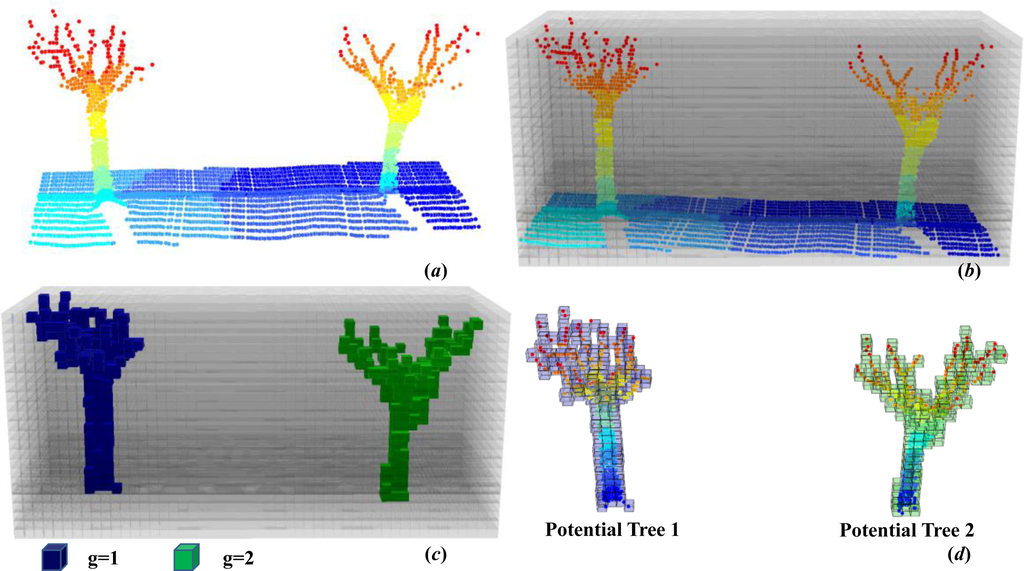
\includegraphics[width=\textwidth]{point_cloud_algorithms/voxel_grid}
	\caption{Voxel grid applied over trees point clouds \cite{Wu2013}}
	\label{fig:point-cloud-algorithms_voxel-grid}
\end{figure}



\subsection{Octrees}

An octrees is a hierarchical space partition technique that adapts its tree data structure to the distribution of points in the cloud. It accomplishes this by recursively dividing each voxel in 8 octants until the tree depth is reached or when there is no more points in that region of space. This can be seen in \cref{fig:point-cloud-algorithms_octree} in which areas with no points have large voxels while areas with high point density have much smaller voxels.

%\afterpage{
\begin{figure}[H]
	\centering
	\begin{minipage}[h]{.495\textwidth}
		\centering
		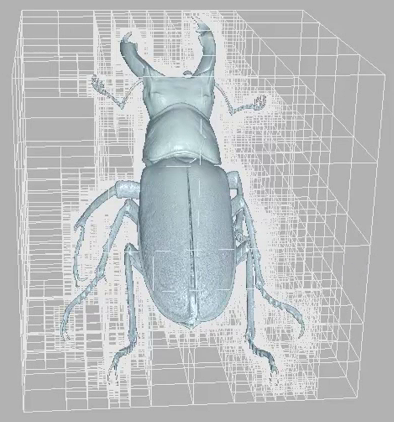
\includegraphics[width=0.55\textwidth]{point_cloud_algorithms/octree_1}
	\end{minipage}\hfill
	\begin{minipage}[h]{.495\textwidth}
		\centering
		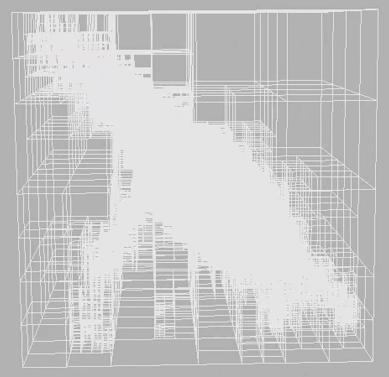
\includegraphics[width=0.6\textwidth]{point_cloud_algorithms/octree_2}
	\end{minipage}
	\caption{Octree of a stag beetle\protect\footnotemark}
	\label{fig:point-cloud-algorithms_octree}
\end{figure}
\footnotetext{\url{http://blog.mpanknin.de/?p=753}}
%}



\subsection{k-d trees}

A k dimensional tree is a space partition technique that can organize points with k dimensions. It is a generic data structure that can be used for 2D and 3D points (examples in \cref{fig:point-cloud-algorithms_2d-tree} and \cref{fig:point-cloud-algorithms_3d-tree}) as well as any other type of data that have an arbitrary number of dimensions (such as point cloud feature descriptors).

The binary k-d tree is built by successively selecting the median point in each axis until all points are inserted in the tree (the selection of the next axis is performed in a circular way, which in the case of three dimensional data means that after processing the z axis, the x axis would be selected).

%\afterpage{
\begin{savenotes}
\begin{figure}[ht]
	\centering
	\begin{minipage}[h]{0.495\textwidth}
		\centering
		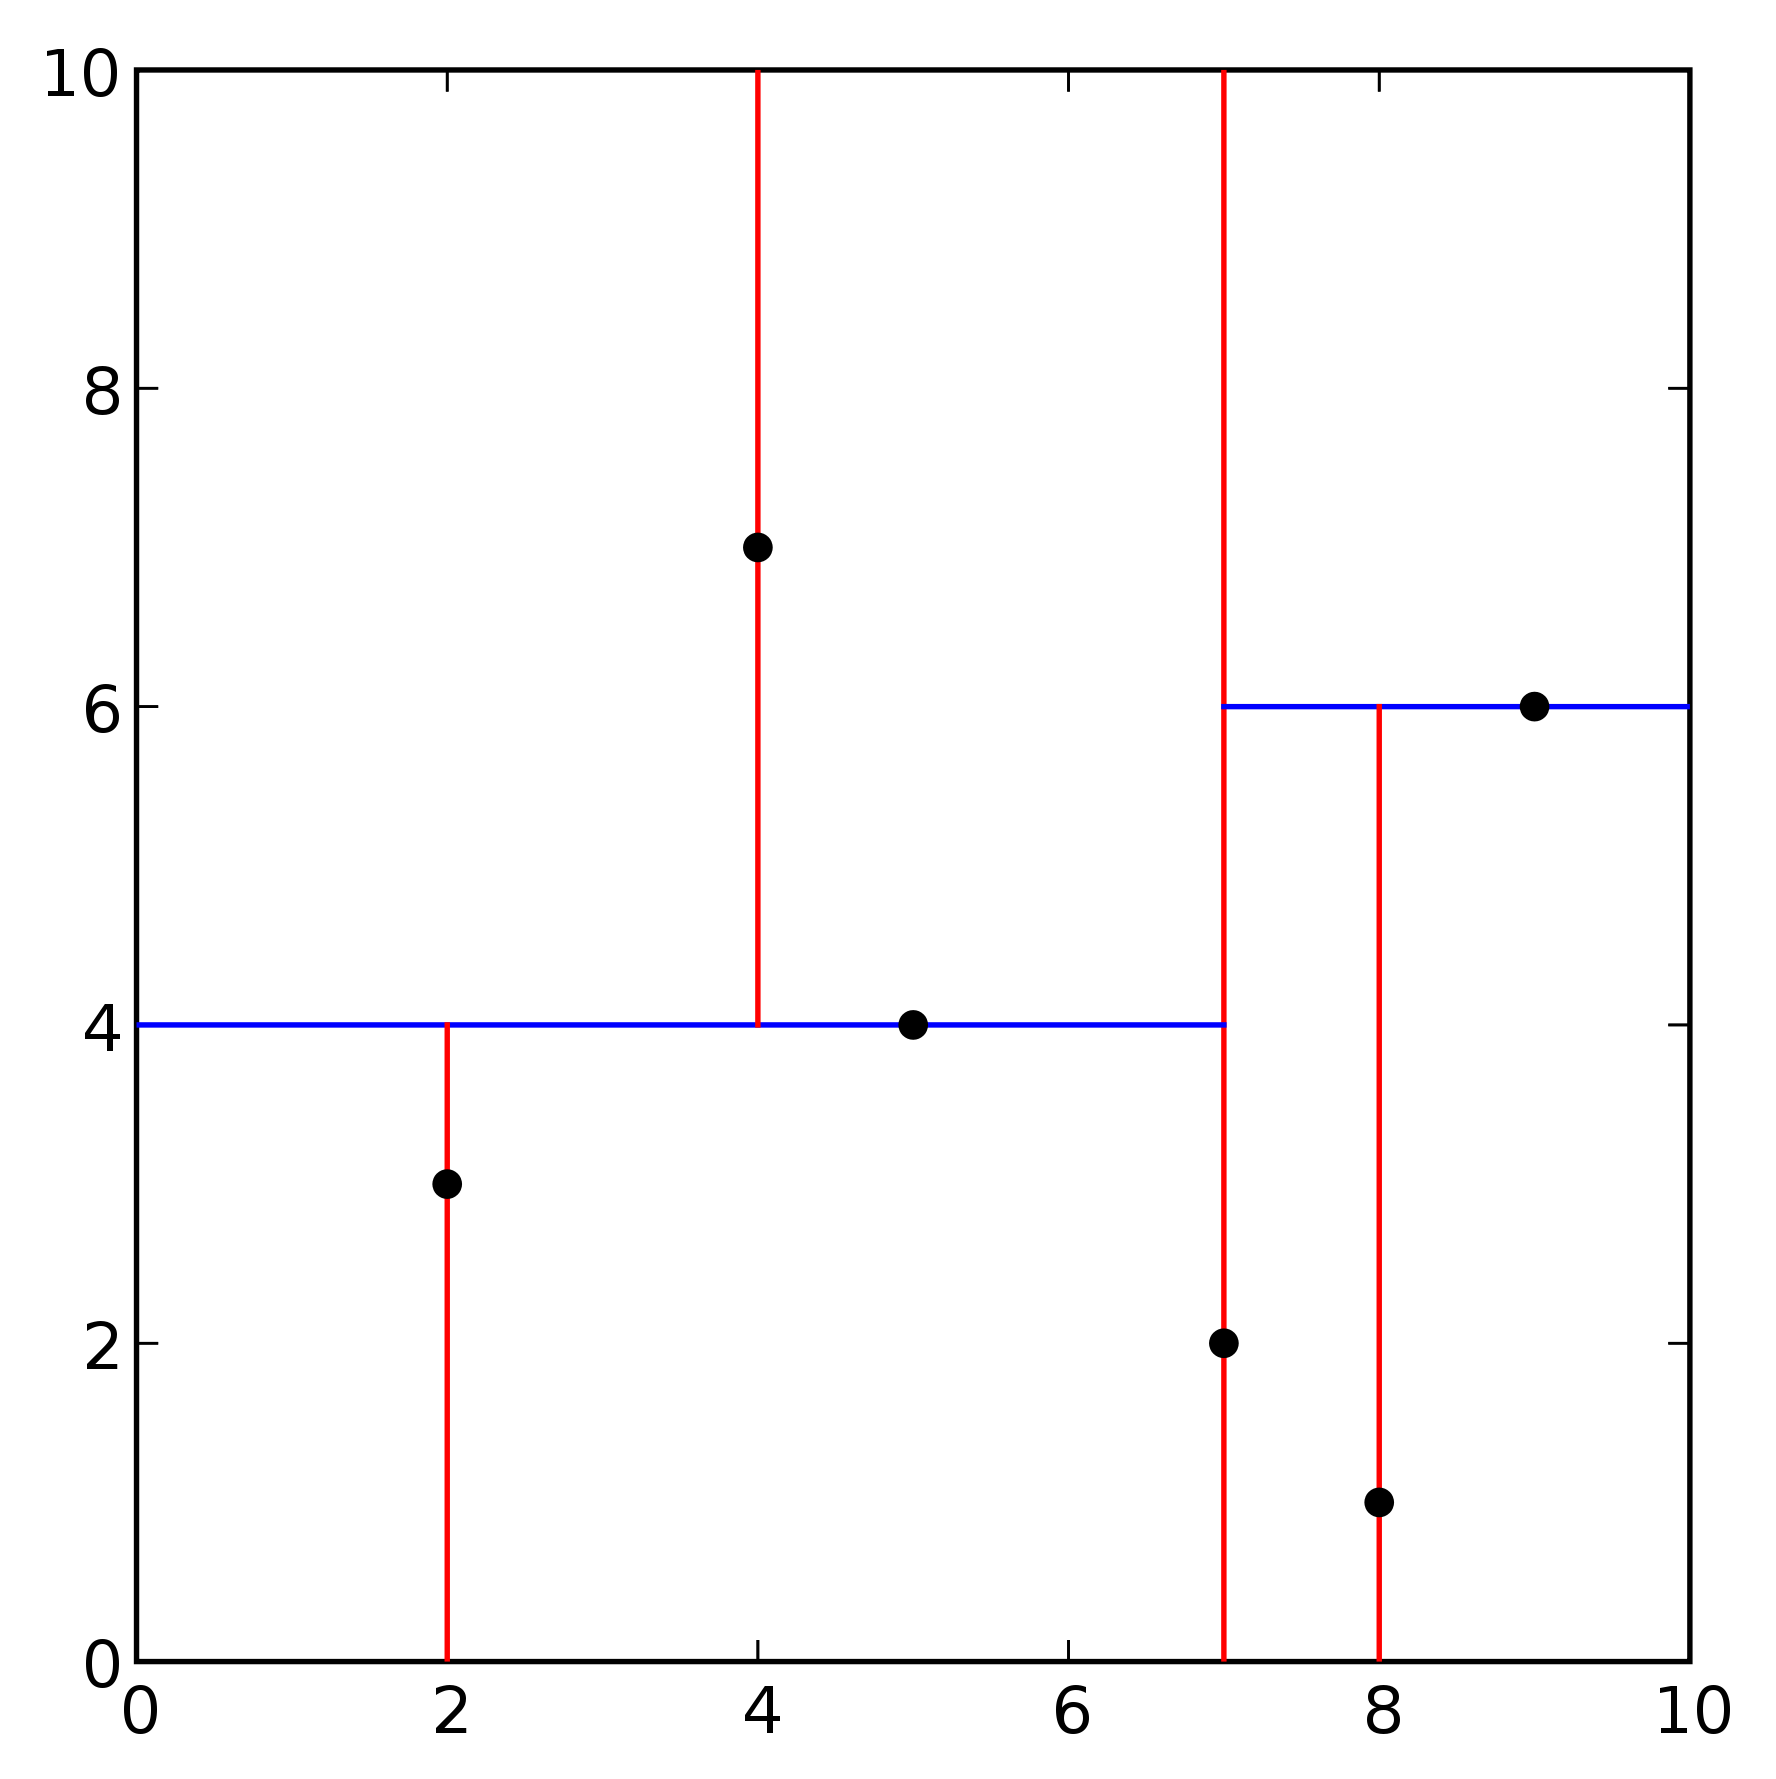
\includegraphics[width=0.6\textwidth]{point_cloud_algorithms/kdtree_2d}
		\caption{2-d tree\protect\footnotemark}
		\label{fig:point-cloud-algorithms_2d-tree}
	\end{minipage}\hfill
	\footnotetext{\url{http://en.wikipedia.org/wiki/K-d_tree}}
	\begin{minipage}[h]{0.495\textwidth}
		\centering
		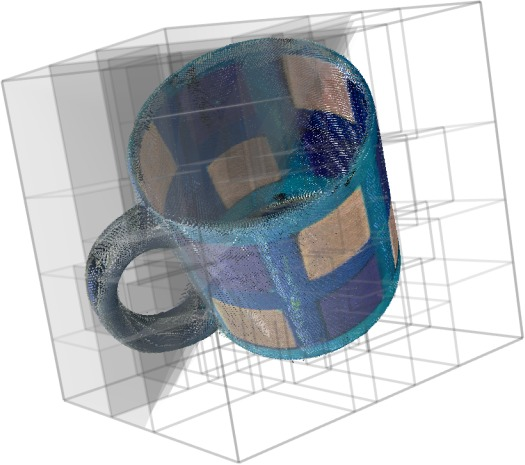
\includegraphics[width=0.65\textwidth]{point_cloud_algorithms/kdtree_3d}
		\caption{3-d tree\protect\footnotemark}
		\label{fig:point-cloud-algorithms_3d-tree}
	\end{minipage}
	\footnotetext{\url{http://docs.pointclouds.org/trunk/group__kdtree.html}}
\end{figure}
\end{savenotes}
%}



\section{Point cloud preprocessing}

Point cloud data that comes from laser sensors can have a considerable amount of noise and an unnecessary level of detail. To cope with these problems, several preprocessing algorithms can be applied, ranging from simple point cloud downsampling to the more advanced outlier removal and surface reconstruction methods.


\subsection{Point cloud downsampling}

Downsampling methods aim to reduce the number of points while maintaining the surface structure of a given point cloud. They can be used to adjust the level of detail according to the point cloud registration precision required.


\subsubsection{Voxel grid sampling}

A voxel grid is a uniform space partition technique that can be used to cluster points according to their Euclidean coordinates. As can be seen in \cref{fig:point-cloud-algorithms_voxel-grid-downsampling}, it is a very effective method to control the level of detail of a point cloud because it gives the ability to specify the maximum number of points that a region in space should have.

The point cloud downsampling is achieved by replacing each cluster with a single point. The selection of this point can be very fast if the voxel center is used, but computing the centroid of the cluster yields better results because it represents the underlying surface with more accuracy and it attenuates errors in the sensors measurements.


%\afterpage{
\begin{figure}[H]
	\centering
	\begin{minipage}[h]{0.495\textwidth}
		\centering
			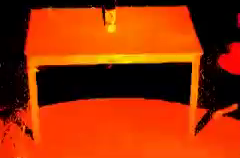
\includegraphics[width=0.78\textwidth]{point_cloud_algorithms/voxel_grid_downsampling_1}
	\end{minipage}\hfill
	\begin{minipage}[h]{.495\textwidth}
		\centering
	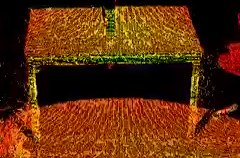
\includegraphics[width=0.78\textwidth]{point_cloud_algorithms/voxel_grid_downsampling_2}
	\end{minipage}
	\caption{Table point cloud before (left) and after (right) voxel grid downsampling\protect\footnotemark}
	\label{fig:point-cloud-algorithms_voxel-grid-downsampling}
\end{figure}
\footnotetext{\url{http://pointclouds.org/documentation/tutorials/voxel_grid.php}}
%}



\subsubsection{Random sampling}

Random sampling \cite{Vitter1984} is a fast downsampling method that randomly selects points from the input cloud until the specified number of samples is reached. This has the advantage of using real measures instead of downsampled approximations, but also means it is more sensible to sensor measurements noise. However, for outdoor environments or very complex scenes, using the real measurements can be preferable than using cluster centroids because the voxels may not have the necessary resolution or may have a prohibitive computational cost.


\subsubsection{Covariance sampling}

Covariance sampling \cite{Gelfand} is a subsampling method that aims to create a stable downsampled point cloud to be registered with \gls{icp} algorithms. It incrementally builds the downsampled point cloud while trying to keep the 6 eigenvalues of the covariance matrix as close to each other as possible.

The resultant point cloud has the desired number of points and is stable enough to be matched with \gls{icp} point to plane algorithms.


\subsection{Outlier removal}

Laser range finders can perform measurements with millimeter accuracy, but they have some limitations that can lead to the creation of outliers \cite{Sotoodeh2006}.

One of those limitations can produce shadow points around objects boundaries. This is due to the fact that a portion of the laser beam may hit the object boundary and other part may hit other areas in the object background. And given that most laser range finders use a weighted sum of several beams, this can yield measurements that are not associated with any real object (outliers). \Cref{fig:point-cloud-algorithms_voxel-grid-downsampling} shows a considerable amount of these shadow points close to the front table legs. Another issue is related to the angle in which the laser beam hits the objects. If the incidence angle is very low, then it may be difficult to detect if the beam had ambient reflections. This can significant increase the measurements noise or even lead to the creation of outliers. Other less common problem is associated with the material properties of the surfaces. For example, objects with very high or very low reflectance, such as metals or glass, can increase the measurements noise. Moreover depending on the combination of surface geometry, material and incidence angle, some objects may even be undetectable by laser range finders.

Given the negative effect that outliers have in object segmentation and registration algorithms, they should be removed in a preprocessing stage. There are several approaches to perform outlier detection and removal \cite{YangZhang2010}, ranging from simple distance thresholds to more robust statistical analysis. The next sections present some of then that can be useful in a localization system.


\subsubsection{Distance filter}

Given that laser range finders have a maximum distance for their measurements, it is wise to remove points that are close or beyond this limit. Moreover, it may be useful to remove points that are too close to the sensor, because they may belong to the robot itself and not the environment.

This can be achieved by applying a minimum and maximum threshold to the distances returned by the laser sensor (before converting then to Euclidean points).


\subsubsection{Passthrough filter}

A passthrough filter can select or remove points according to their properties.

For outlier removal, it can be used to select points that are within a given bounding box (useful when we already know what area of the environment we want to analyze) or remove points that don't have the appropriate intensity or color.


\subsubsection{Radius outlier removal filter}

The radius outlier removal filter deletes points that don't have a minimum number of neighbors within a specified radius distance. It can be useful when the point density is known and is very effective in removing isolated points.


\subsubsection{Statistical outlier removal filter}

The statistical outlier removal filter \cite{Rusu2010a} performs a global analysis of the distances between points and discards the ones that don't follow the global distance distribution.

It is a robust filter that adapts itself to the point cloud density and is very effective in removing shadow points. To do so, it computes the mean distance that each point has to a given number of neighbors and builds a global distance distribution (example in \cref{fig:point-cloud-algorithms_statistical-outlier-removal}). Then, assuming that the distribution is Gaussian, it discards the points that have a distance higher than a given threshold (that is a percentage of the standard deviation of the distance distribution).

%\afterpage{
\begin{figure}[H]
	\centering
	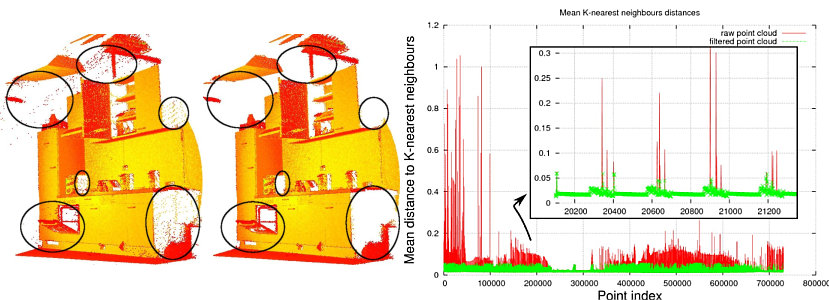
\includegraphics[width=\textwidth]{point_cloud_algorithms/statistical_outlier_removal}
	\caption{Statistical outlier removal filter\protect\footnotemark}
	\label{fig:point-cloud-algorithms_statistical-outlier-removal}
\end{figure}
\footnotetext{\url{http://pointclouds.org/documentation/tutorials/statistical_outlier.php}}
%}


\subsection{Surface and object reconstruction and resampling}

Depending on the level of sensor noise and amount of outliers present in a given point cloud, it may be necessary to employ surface reconstruction techniques to fill gaps in sensor data or correct measurements errors. The next sections introduce some of the most common techniques to achieve these goals.


\subsubsection{Object recognition and model fitting}

One of the most advanced techniques that can be used to fill gaps in sensor data relies on object recognition or model fitting. These techniques are usually applied to small objects that have only the front side visible. They are useful when it is necessary to know the approximate shape of objects. However, they require a priori knowledge about the types of shapes or objects that are present in the scene.


\subsubsection{Moving Least Squares}\label{sec:point-cloud-algorithms_mls}

Moving least squares \cite{Alexa2003} is a surface reconstruction algorithm that uses higher order bivariate polynomials to fit surfaces to a given set of points. It can be used to fill possible gaps in sensor data, smooth the point cloud (shown in \cref{fig:point-cloud-algorithms_mls-smoothing}), refine surface normals (shown in \cref{fig:point-cloud-algorithms_mls-nomal-refinement}) and perform downsampling or upsampling.

Surface reconstruction can also be useful when the point cloud is built from several laser scans with different origins and registered with some alignment errors. In \cref{fig:point-cloud-algorithms_mls-nomal-refinement} can be seen that the normal estimation is not very accurate in the regions of overlap between different scans. This can be solved by estimating the normals using the surfaces computed by the moving least squares algorithm instead of using the point's neighbors.


%\afterpage{
\begin{figure}[H]
	\centering
	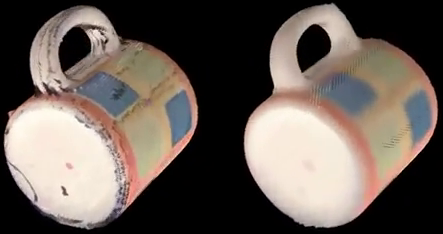
\includegraphics[width=0.57\textwidth]{point_cloud_algorithms/mls_smoothing}
	\caption{Surface smoothing using moving least squares algorithm\protect\footnotemark}
	\label{fig:point-cloud-algorithms_mls-smoothing}
\end{figure}
\footnotetext{\url{http://pointclouds.org/documentation/tutorials/resampling.php}}
%}

%\afterpage{
\begin{figure}[H]
	\centering
	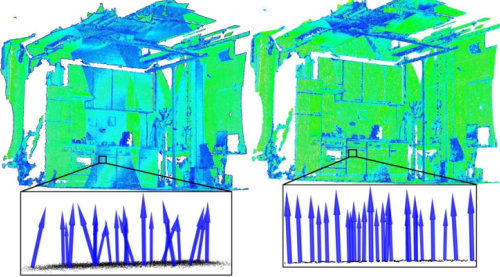
\includegraphics[width=0.57\textwidth]{point_cloud_algorithms/mls_nomal_refinement}
	\caption{Surface normals refinement using moving least squares algorithm \cite{Rusu2010a}}
	\label{fig:point-cloud-algorithms_mls-nomal-refinement}
\end{figure}
%}



\section{Point cloud features}

Aligning two point clouds with overlapping views of the environment requires the establishment of point correspondences. If both point clouds have similar sensor origins, these can be determined with nearest neighbor's searches and filtered with correspondence rejectors (using other point properties such as reflectance and color). But if they were acquired in two very different positions, then more advanced techniques must be employed.

One of those techniques uses histograms to describe the geometric properties of the environment around a given point. This allows points to be matched even if they have completely different Euclidean coordinates. Also, by using histograms and sampling techniques, these descriptors are much more robust against sensor noise and varying level of point density. However, these advantages come with a heavy computational cost, and as such, point descriptors should only be computed on the most descriptive areas of the environment.

Identifying these environment points is known as feature / keypoint detection, and usually involves finding interesting points, such as corners and edges. Besides uniqueness, these points must also be repeatable. This means that the detection algorithms should be able to find the same points even if they are present in different point clouds with sensor noise and varying point density. This is of the utmost importance, because if the same keypoints are not identified on both clouds, then matching the point descriptors will likely fail.

The next sections introduce some of the most used algorithms for normal estimation, keypoint detection and point description.


\subsection{Surface normal estimation}

Surface normals provide information about the orientation of their underlying geometry and are widely used as the basis for other point descriptors. They can be computed using plane fitting methods or using more advanced techniques such as the one presented in \cref{sec:point-cloud-algorithms_mls}.

These algorithms analyze the neighborhood of a given point in order to compute the surface normal, and as such, the correct specification of what points should be included in the estimation is crucial to achieve accurate results. This depends on the environment geometry and the level of detail that is required, and is usually done by specifying a radius distance (example in \cref{fig:point-cloud-algorithms_surface-normals}) or by limiting the number of neighbor points to use.

\begin{figure}[H]
	\centering
	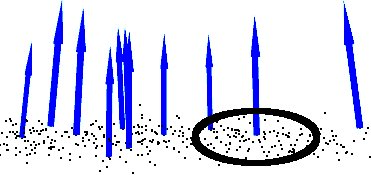
\includegraphics[width=0.5\textwidth]{point_cloud_algorithms/surface_normals}
	\caption{Point neighborhood for normal estimation \cite{Rusu2010a}}
	\label{fig:point-cloud-algorithms_surface-normals}
\end{figure}


\chapter{Localization system} \label{chap:localization-system}



\section*{}

FF



\section{FF}

FF

\chapter{Localization system evaluation} \label{chap:localization-system-evaluation}



\section*{}

FF



\section{FF}

FF

\chapter{Conclusions} \label{chap:conclusions-and-future-work}



\section*{}

The proposed localization system is able to maintain pose tracking with less 1-2 centimeters of translation error and less than a 1-3 degrees of rotation error (in 3 and 6 DoF respectively) with the sensors moving at several velocities even in cluttered and dynamic environments. Moreover, when tracking is lost or no initial pose is given, the system is able to find a valid global pose estimate by switching to more robust registration algorithms that use feature matching. This approach achieved fast pose tracking and reliable initial pose estimation while also providing the set of the accepted initial poses before registration refinement, which can be very valuable information for a navigation supervisor when the robot is in an ambiguous region that can be registered in similar zones of the known map. The system also allows dynamic reconfiguration of the number of laser scans to assemble in order to mitigate laser measurement errors and can adapt its rate of operation according to the robot estimated velocity.

The sub-centimeter accuracy achieved by the proposed localization system along with the dynamic map update capability and the need of no artificial landmarks / ambient modifications will allow the fast deployment of mobile robots capable to operate safely and accurately in cluttered environments.



\section{Main contributions}

The following list gives an overview of the main contributions of the presented work:

\begin{itemize}
	\item A \gls{lidar} assembler\footnote{\url{https://github.com/carlosmccosta/laserscan_to_pointcloud}} capable of:
	\begin{itemize}
		\item Merging measurements from several sensors
		\item Dynamic adjust its configurations based on the speed of the robot in order to merge more scans when the robot is moving slower
		\item Use spherical linear interpolation to reduce scan deformation
		\item Emulate a 3D sensor when the \gls{lidar} is mounted on a tilting platform
	\end{itemize}

	\item An localization system\footnote{\url{https://github.com/carlosmccosta/dynamic_robot_localization}} that:
	\begin{itemize}
		\item Is efficient, modular and extensible to new 3/6 \gls{dof} algorithms
		\item Can dynamically and incrementally update the localization map
		\item Provides the set of acceptable initial poses when reseting tracking (useful for localization supervisors)
		\item Gives several localization quality metrics such as percentage, \gls{rmse} and angular distribution of the correctly registered points
		\item Gives the possibility to use 3 different point cloud registration algorithms based on the tracking state (normal tracking, tracking recovery, initial pose estimation)
	\end{itemize}

	\item Development of a testing infrastructure to automate the collection, analysis and generation of localization results

	\item 3 \gls{dof} Localization datasets\footnote{\url{https://github.com/carlosmccosta/dynamic_robot_localization_tests}}:
	\begin{itemize}
		\item 4 datasets with subcentimeter ground truth in static and dynamic environments using a robot moving at different speeds
		\item 6 Gazebo and 6 Stage simulation datasets
		\item Improvement of external 3/6 \gls{dof} datasets (ground truth time synchronization and laser transformations calibration)
	\end{itemize}

	\item Test of the localization system on public datasets and comparison with:
	\begin{itemize}
		\item Ground truth systems from three different testing environments
		\item Widely used localization systems (\gls{amcl} and ethzasl-icp-mapper)
		\item Well known \gls{slam} system (GMapping)
	\end{itemize}
 	
	\item In the context of the \gls{carlos} project:
	\begin{itemize}
		\item The robot hardware configuration proved adequate for the intended tasks and environment
		\item The 3 \gls{dof} localization system was able to run in real time on the low computational power on-board computer
	\end{itemize}
\end{itemize}



\section{Future work}

The current implementation of the self-localization system can be further improved with \gls{gpu} support \cite{Tamaki2010} in order to achieve higher update rates in 6 \gls{dof} and also with loop closing algorithms \cite{Grisetti2012} in order to become a complete \gls{slam} system and allow the creation of accurate maps of very large environments. Moreover, it could be extended to support image based localization \cite{Labb2014} and semantic perception and mapping of the environment \cite{Santos2013}.





%---------------------------------------------------------------------------------------------------
% Appendixes, bibliography and index
%---------------------------------------------------------------------------------------------------

\appendix
\chapter{Appendix 1} \label{app:appendix1}



\section*{}

FF



\section{FF}

FF


\PrintBib{references/references}
%\PrintIndex


\end{document}
